\section{ETCS Kernel Overview}\label{s:ETCS_Kernel_Overview}

The ETCS Kernel module consists of the 13 functional components, i.e. F2.1 to F2.13 as depicted in Figures~\ref{f:f2.1_overview} to \ref{f:f2.13_overview}. Note that due to the complexity of the Kernel module the SysML diagram has been splitted into 13 figures. Each of the figures shows one of the subcomponents F2.1 to F2.13 and its connections to the other components in F2 and the inputs respectively outputs of F2. In the following we briefly describe the functionality of these components.
\begin{description}
\item[F2.1: Manage\_TrackSideInformation\_Integration] This component is responsible for receiving Eurobalise telegrams and Euroradio messages from the API and performs several consistency checks on the inputs. The corresponding SysML diagram is shown in Figure~\ref{f:f2.1_overview}. For further details we refer to Section~\ref{s:F2.1}.

\item[F2.2: Manage\_ETCS\_Procedures] This component describes the Start of Mission procedure of the train until the current status will change to another mode, level or other procedure. The corresponding SysML diagram is shown in Figure~\ref{f:f2.2_overview}. For further details we refer to Section~\ref{s:F2.2}.

\item[F2.3: trainData] Implementation of the train data with the corresponding interfaces to  driver and RBC. The corresponding SysML diagram is shown in Figure~\ref{f:f2.3_overview}. For further details we refer to Section~\ref{s:F2.3}.

\item[F2.4: TrackAtlas] Implementation of the track database as a function of the evc.  The corresponding SysML diagram is shown in Figure~\ref{f:f2.4_overview}. For further details we refer to Section~\ref{s:F2.4}.

\item[F2.5: ManageLevelAndMode] Defines the behaviour of Modes and Levels transitions. The corresponding SysML diagram is shown in Figure~\ref{f:f2.5_overview}. For further details we refer to Section~\ref{s:F2.5}.

\item[F2.6: calculateTrainPosition] The purpose of this component is to calculate the locations of linked and unlinked balise groups and the current train position while the train is running along the track. The corresponding SysML diagram is shown in Figure~\ref{f:f2.6_overview}. For further details we refer to Section~\ref{s:F2.6}.


\item[F2.7: SpeedSupervision\_Integration] This component monitors the current speed of the train and its location to ensure that the speed remains within the given speed and distance limits. The corresponding SysML diagram is shown in Figure~\ref{f:f2.7_overview}. For further details we refer to Section~\ref{s:F2.7}.


\item[F2.8: Provide\_Position\_Report] The component builds a position report for the RBC, i.e., message 132, and provides it as an output. The corresponding SysML diagram is shown in Figure~\ref{f:f2.8_overview}. For further details we refer to Section~\ref{s:F2.8}.


\item[F2.9: Manage\_Radio\_Communication] This component implements the onboard management of a single communication session with the track, i.e.~a single RBC. It controls the establishment, maintenance and termination process of a radio communication session and steers the underlying communication safety layer as well as the mobile device. Those and the data transfer itself are not part of this component. The corresponding SysML diagram is shown in Figure~\ref{f:f2.9_overview}. For further details we refer to Section~\ref{s:F2.9}.


\item[F2.10: manageDMI\_input] This component handles messages respectively data coming from the Driver Machine Interface (DMI) to the ETCS OBU. The corresponding SysML diagram is shown in Figure~\ref{f:f2.10_overview}. For further details we refer to Section~\ref{s:F2.10}.


\item[F2.11: manageDMI\_output] This component handles messages respectively data being send from the ETCS OBU to the DMI. The corresponding SysML diagram is shown in Figure~\ref{f:f2.11_overview}. For further details we refer to Section~\ref{s:F2.11}.


\item[F2.12: manageTIU\_input] This component handles messages respectively data coming from the Train Interface Unit (TIU) to the ETCS OBU. The corresponding SysML diagram is shown in Figure~\ref{f:f2.12_overview}. For further details we refer to Section~\ref{s:F2.12}.


\item[F2.13: manageTIU\_output] This component handles messages respectively data being send from the ETCS OBU to the TIU. The corresponding SysML diagram is shown in Figure~\ref{f:f2.13_overview}. For further details we refer to Section~\ref{s:F2.13}.
\end{description}

\begin{figure}
\center
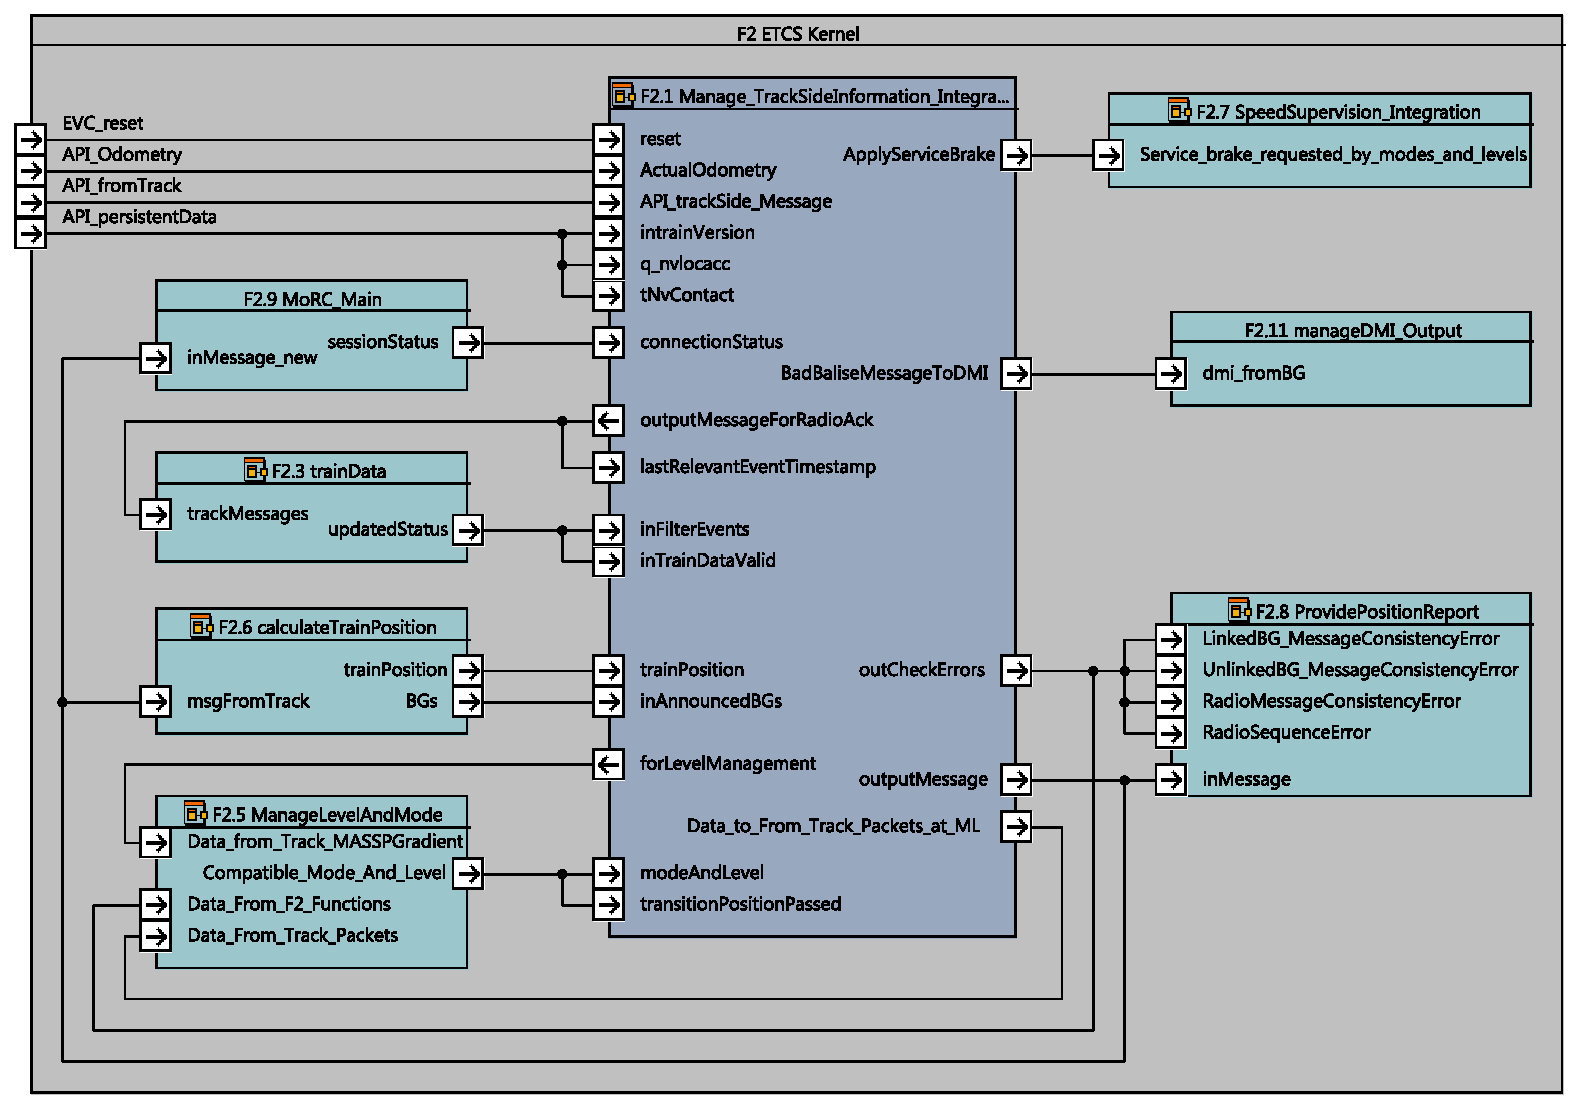
\includegraphics[width=\textwidth]{F2_F2_1.pdf}
\caption{F2: ETCS Kernel SysML diagram with focus on F2.1 Manage\_TrackSideInformation\_Integration component.}\label{f:f2.1_overview}
\end{figure}

\begin{figure}
\center
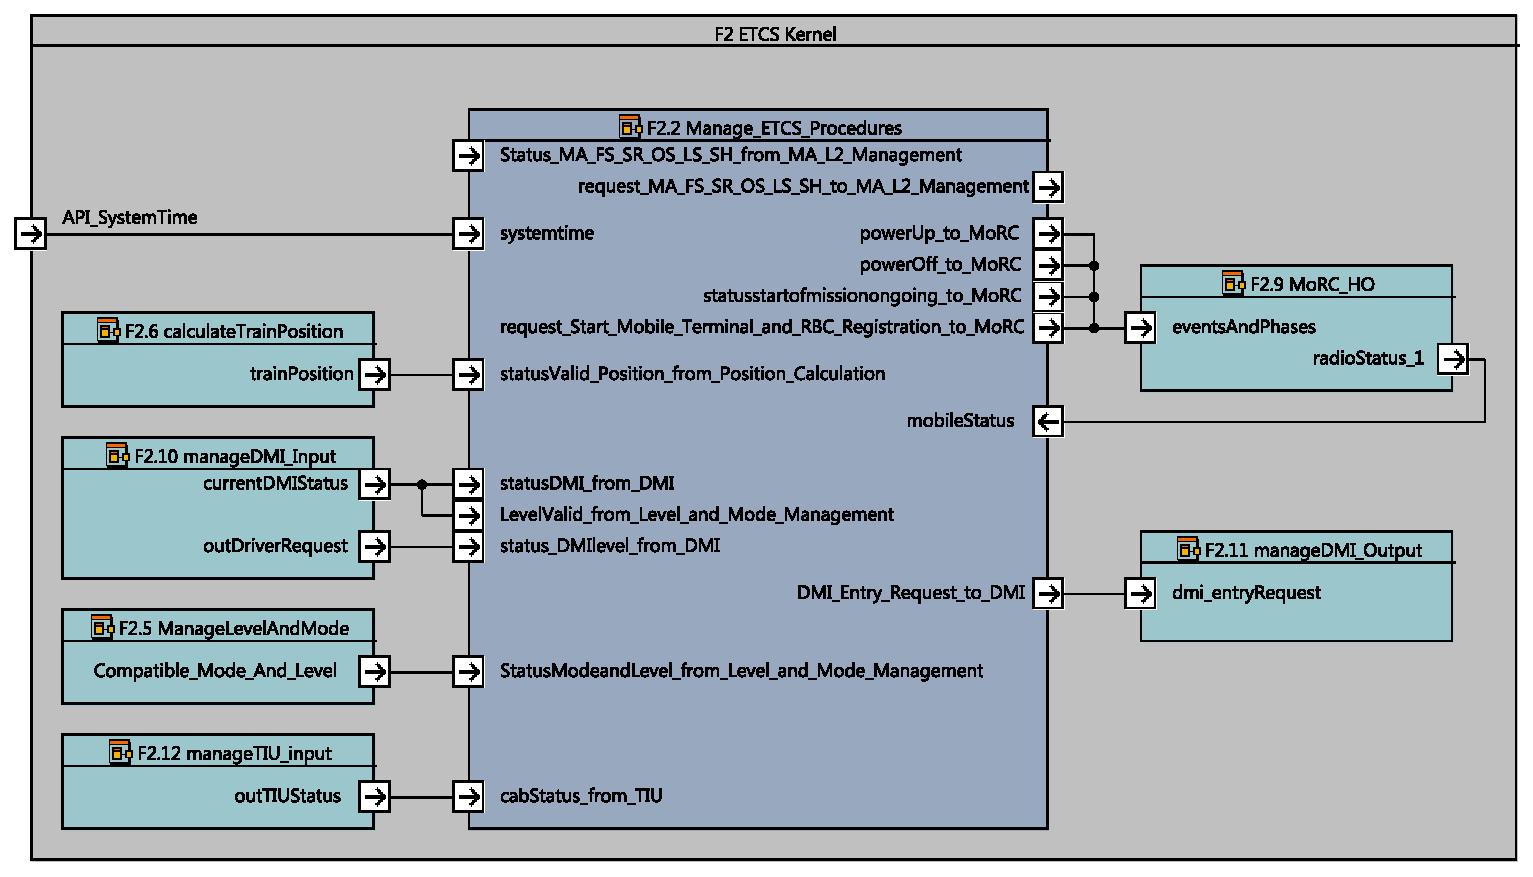
\includegraphics[width=\textwidth]{F2_F2_2.pdf}
\caption{F2: ETCS Kernel SysML diagram with focus on F2.2 Manage\_ETCS\_Procedures component.}\label{f:f2.2_overview}
\end{figure}

\begin{figure}
\center
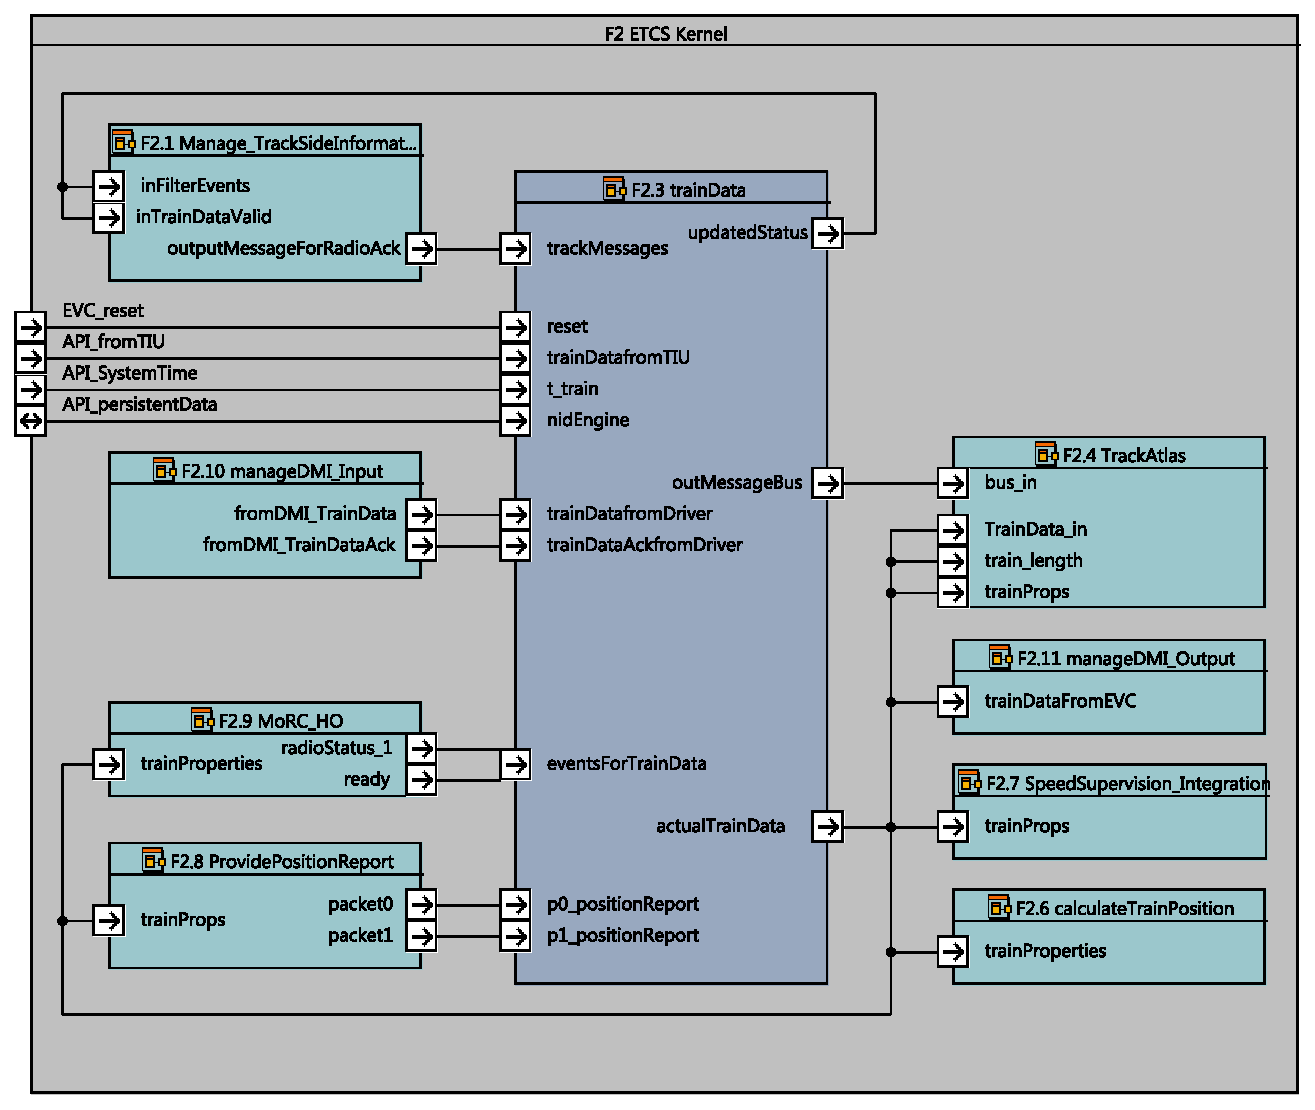
\includegraphics[width=\textwidth]{F2_F2_3.pdf}
\caption{F2: ETCS Kernel SysML diagram with focus on F2.3 trainData component.}\label{f:f2.3_overview}
\end{figure}

\begin{figure}
\center
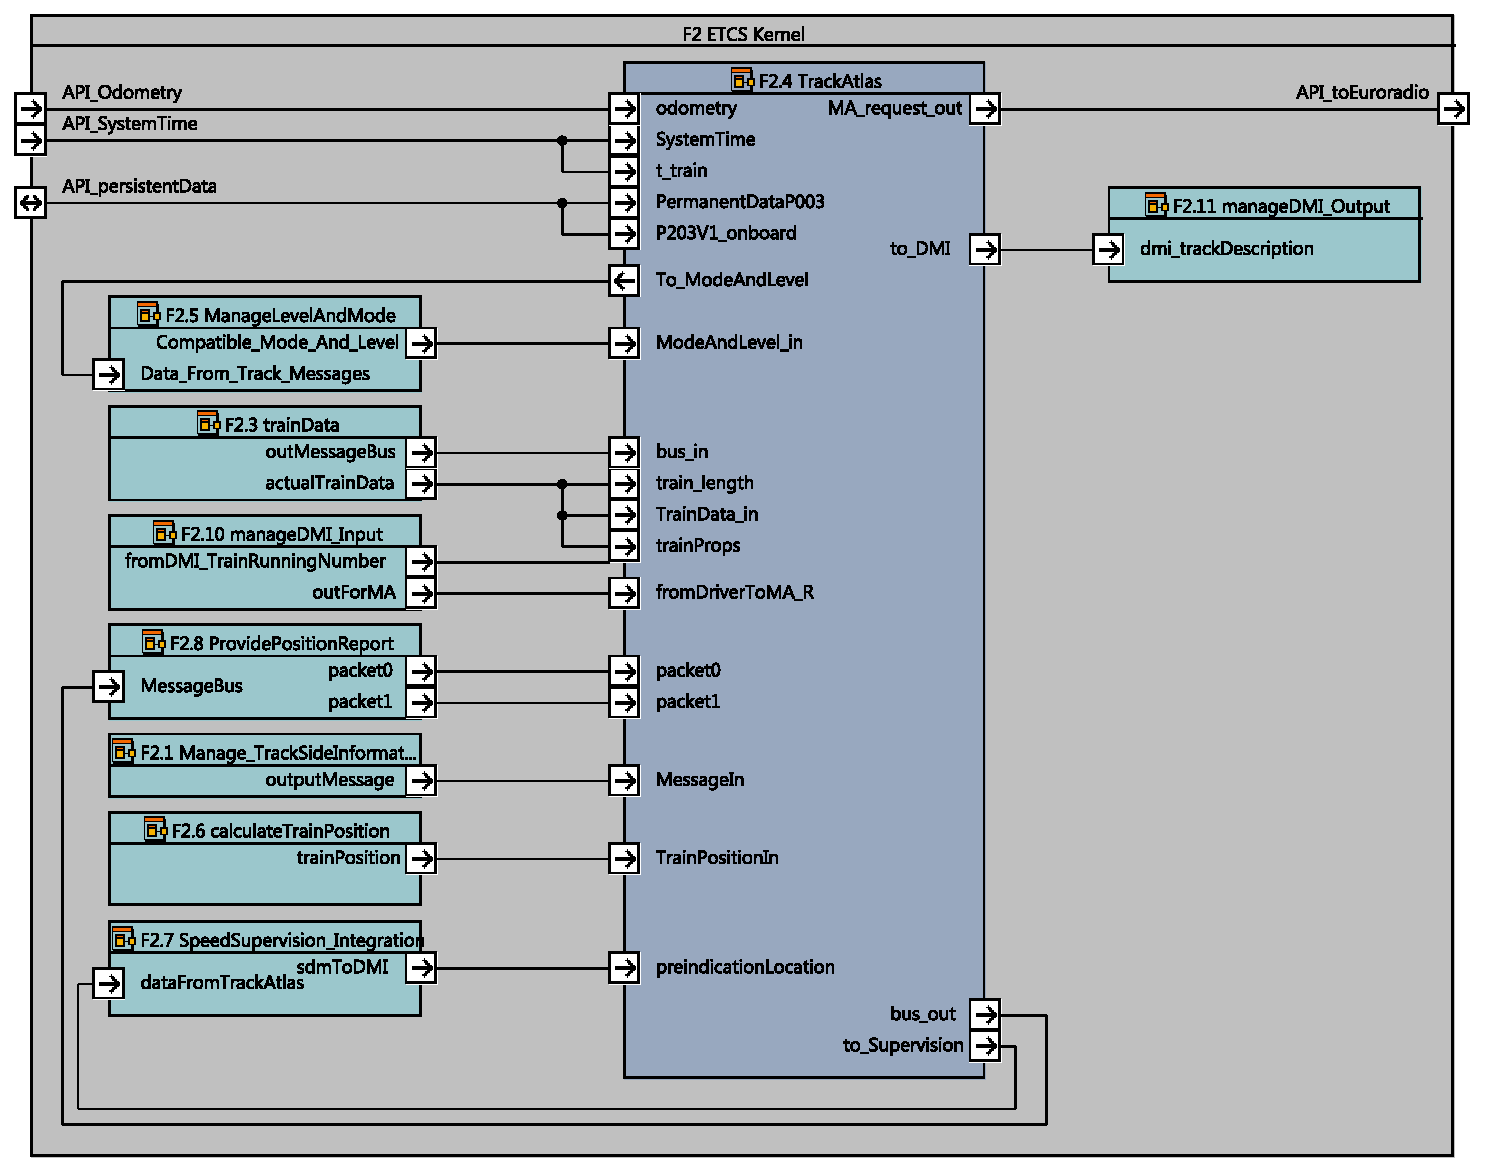
\includegraphics[width=\textwidth]{F2_F2_4.pdf}
\caption{F2: ETCS Kernel SysML diagram with focus on F2.4 TrackAtlas component.}\label{f:f2.4_overview}
\end{figure}

\begin{figure}
\center
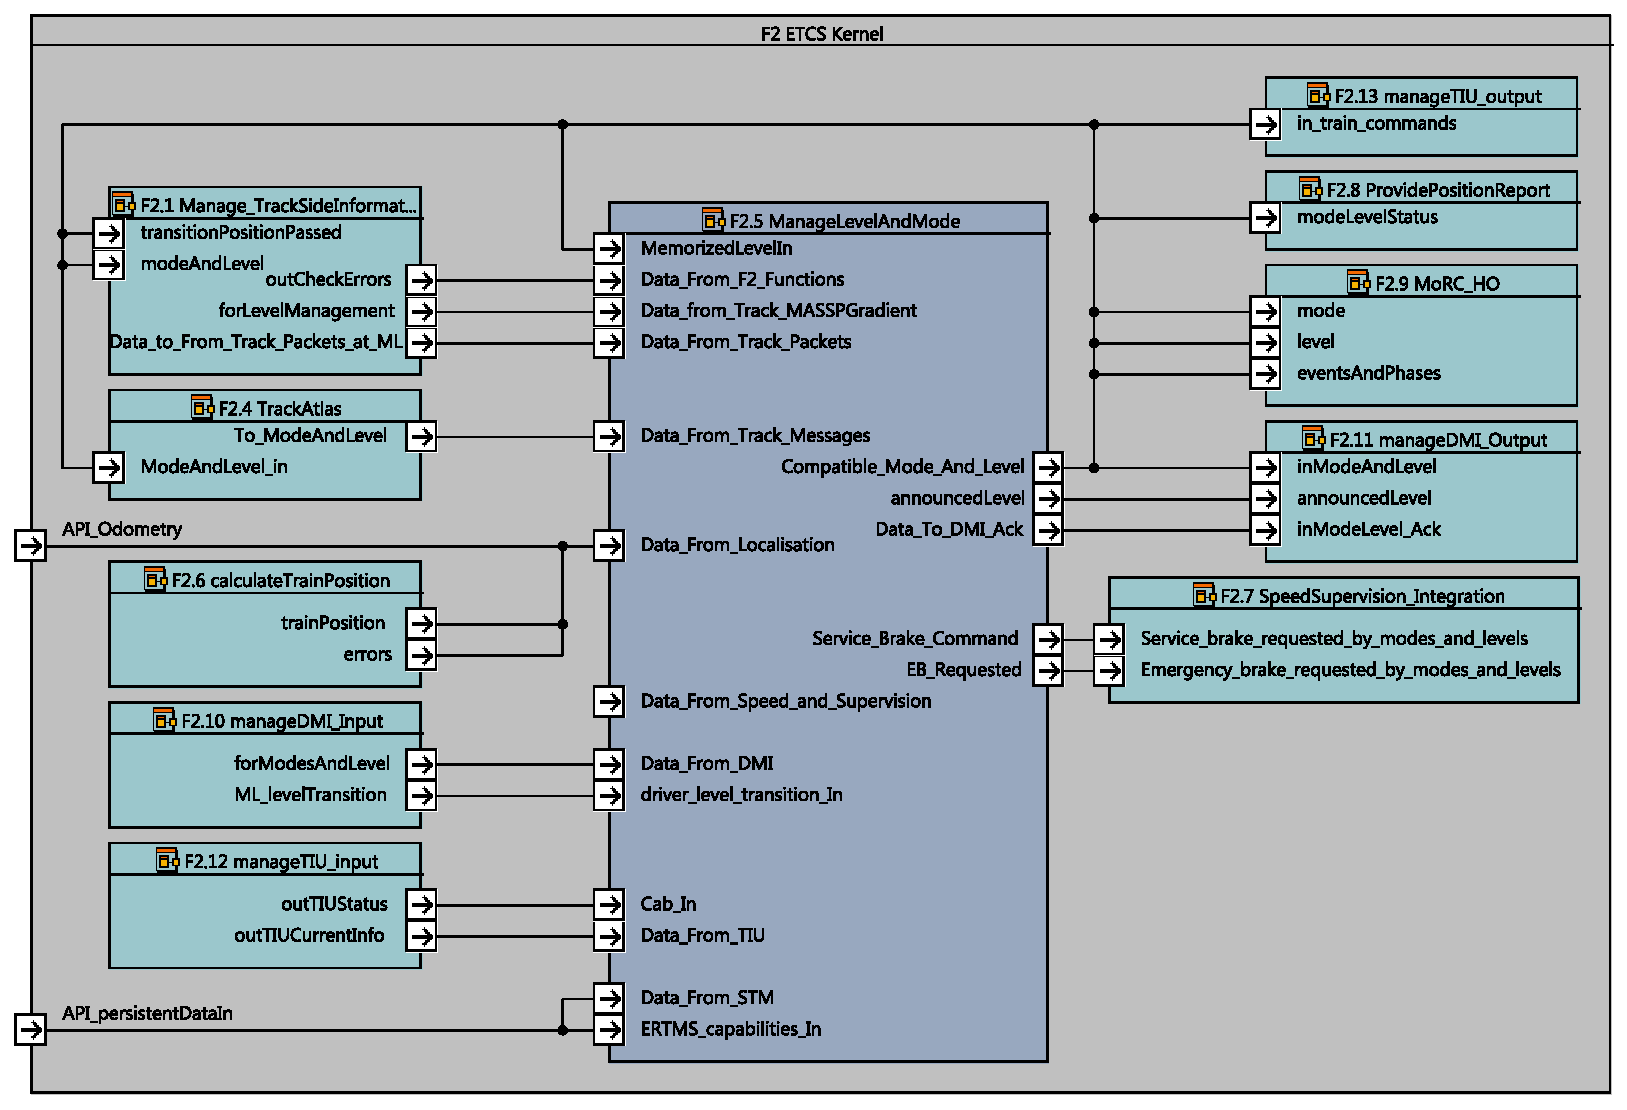
\includegraphics[width=\textwidth]{F2_F2_5.pdf}
\caption{F2: ETCS Kernel SysML diagram with focus on F2.5 Mode\_and\_Level component.}\label{f:f2.5_overview}
\end{figure}

\begin{figure}
\center
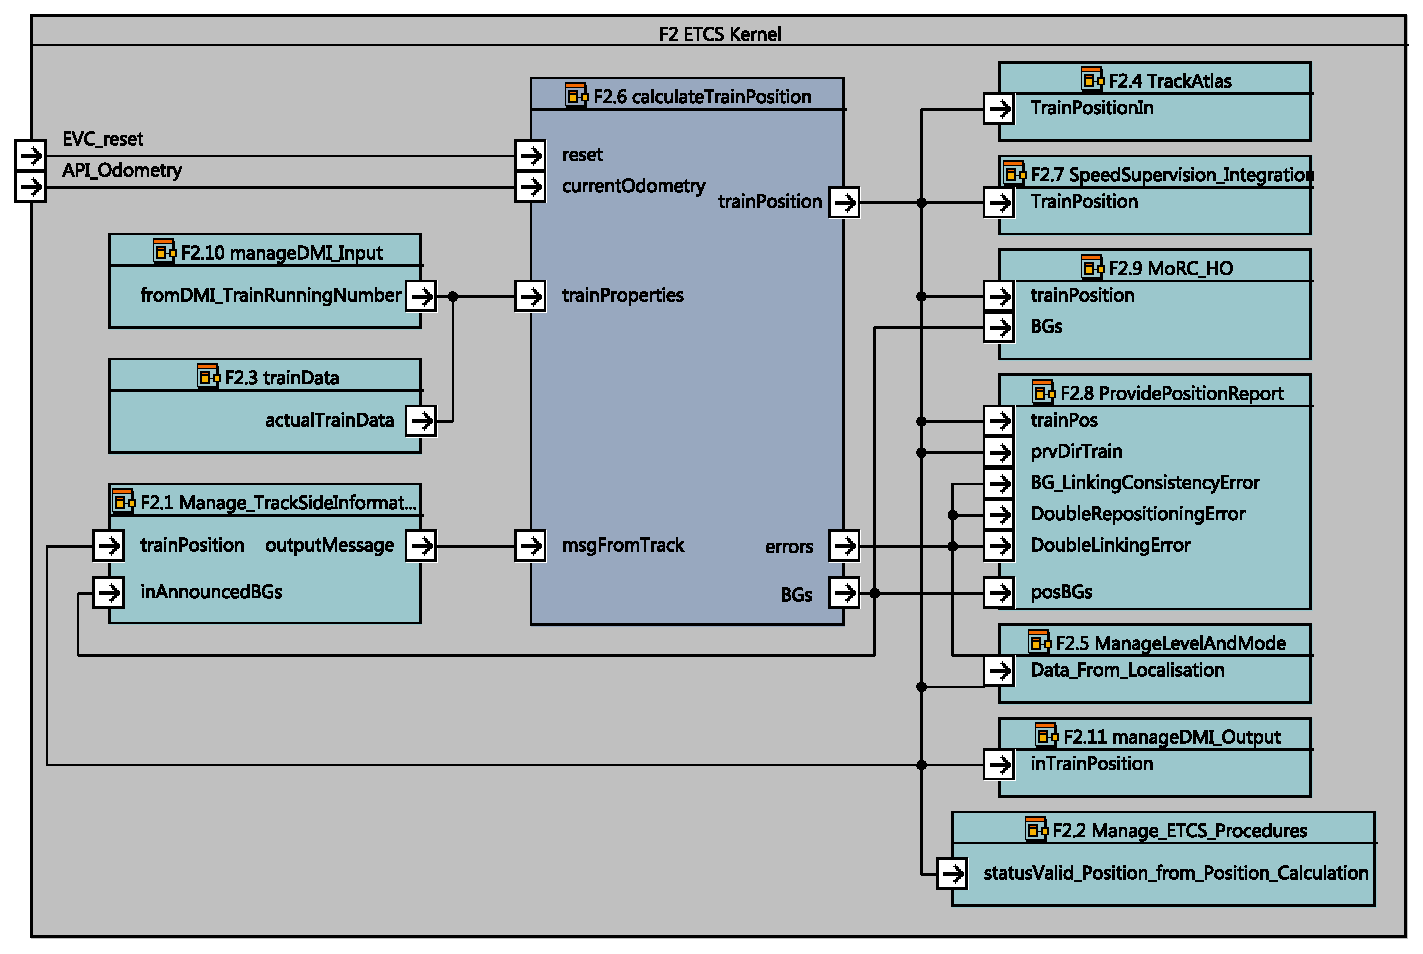
\includegraphics[width=\textwidth]{F2_F2_6.pdf}
\caption{F2: ETCS Kernel SysML diagram with focus on F2.6 calculateTrainPosition component.}\label{f:f2.6_overview}
\end{figure}

\begin{figure}
\center
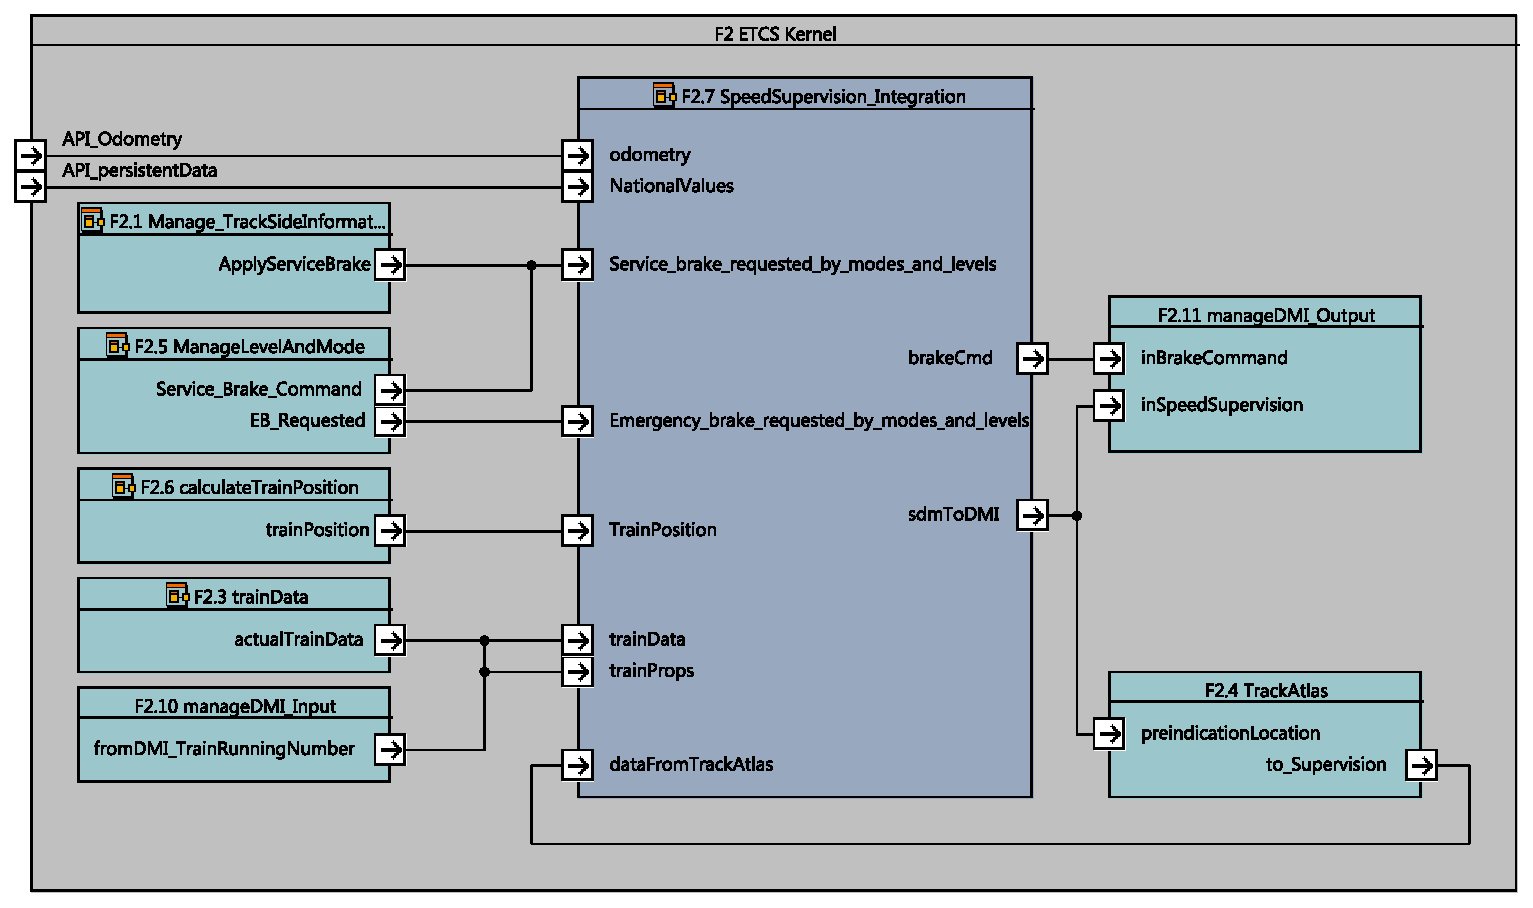
\includegraphics[width=\textwidth]{F2_F2_7.pdf}
\caption{F2: ETCS Kernel SysML diagram with focus on F2.7 SpeedSupervision\_Integration component.}\label{f:f2.7_overview}
\end{figure}

\begin{figure}
\center
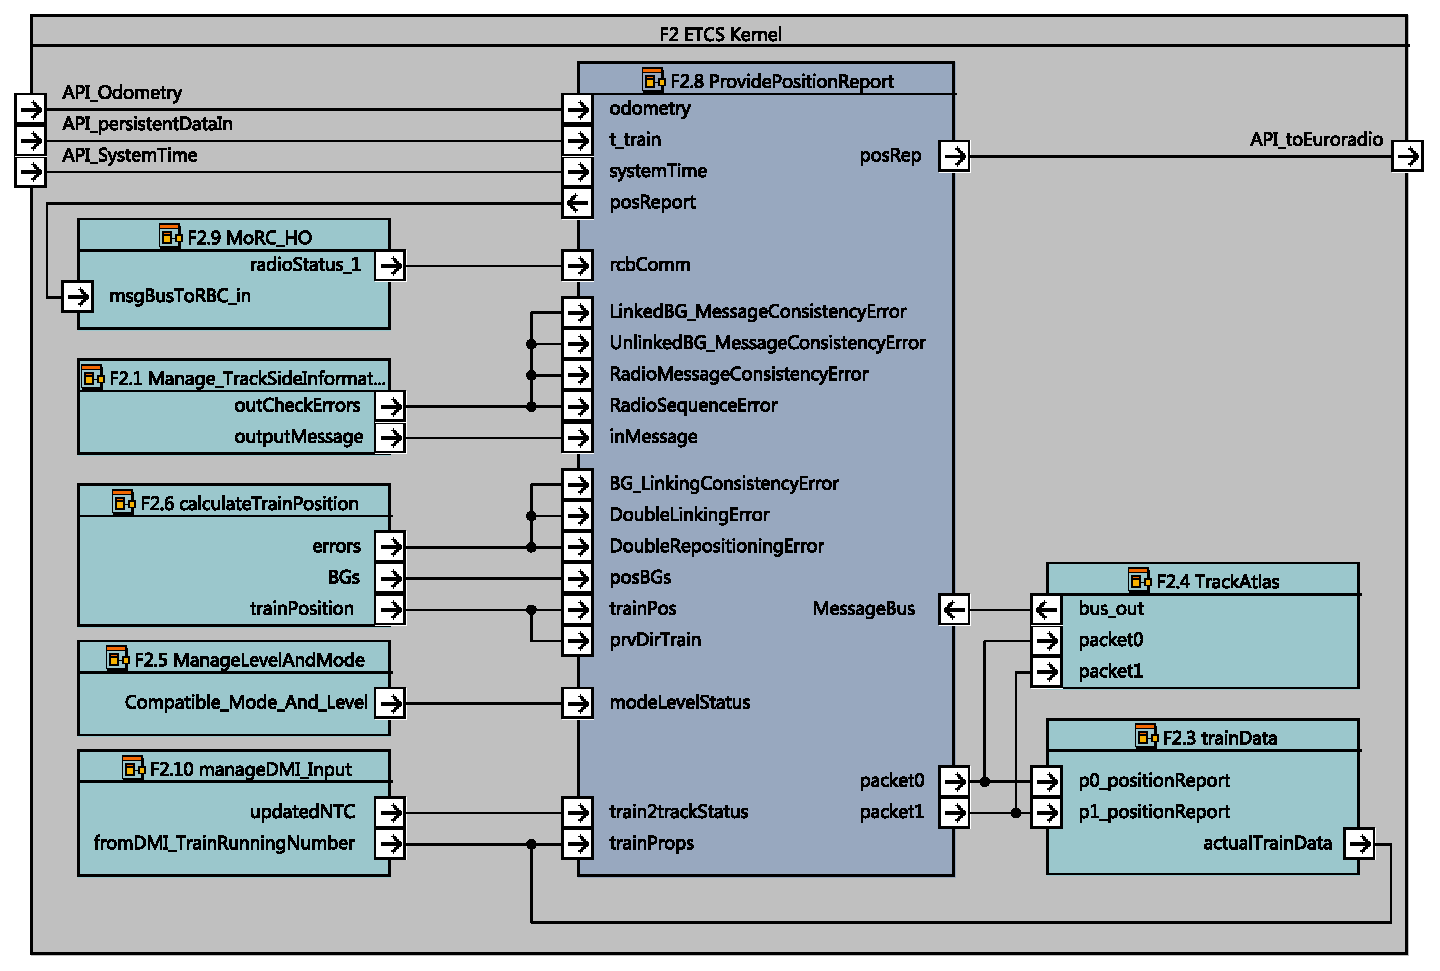
\includegraphics[width=\textwidth]{F2_F2_8.pdf}
\caption{F2: ETCS Kernel SysML diagram with focus on F2.8 Provide\_Position\_Report component.}\label{f:f2.8_overview}
\end{figure}

\begin{figure}
\center
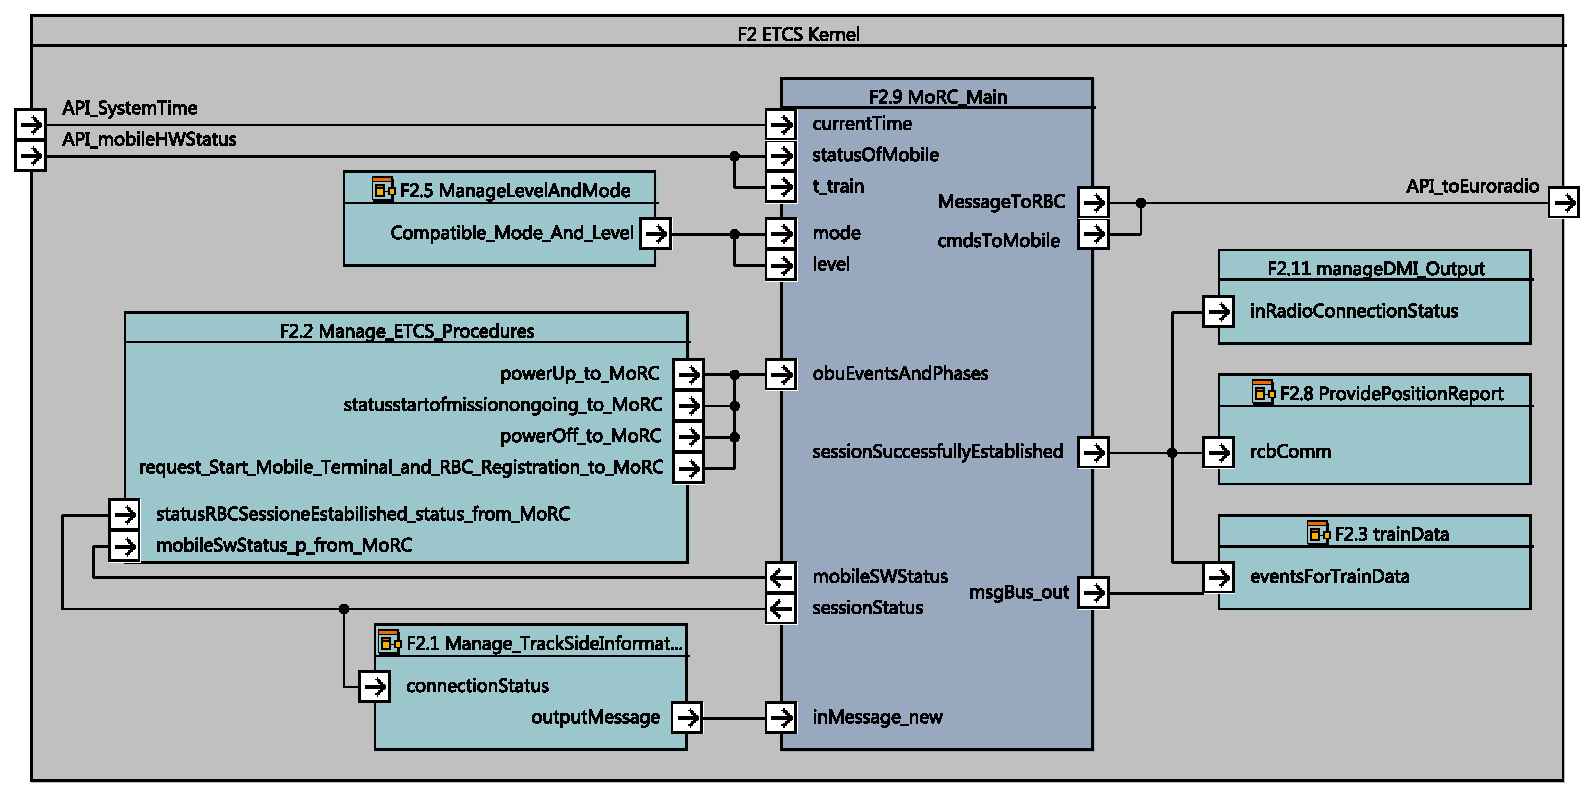
\includegraphics[width=\textwidth]{F2_F2_9.pdf}
\caption{F2: ETCS Kernel SysML diagram with focus on F2.9 Manage\_Radio\_Communication component.}\label{f:f2.9_overview}
\end{figure}

\begin{figure}
\center
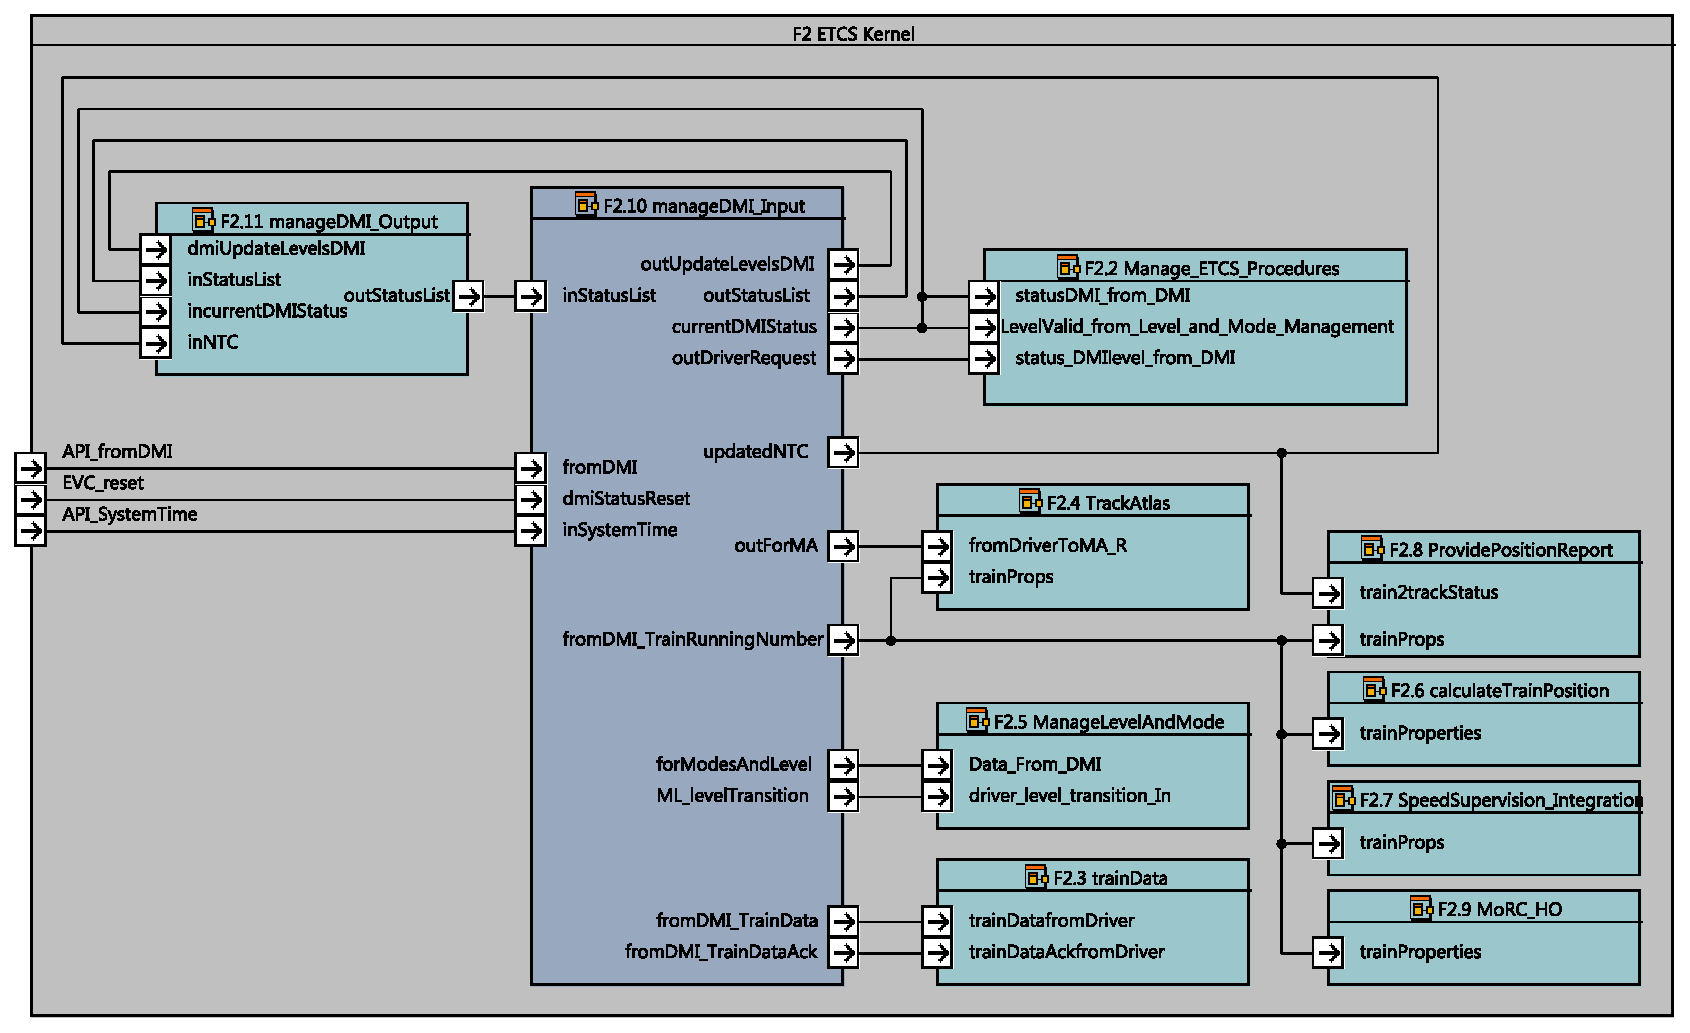
\includegraphics[width=\textwidth]{F2_F2_10.pdf}
\caption{F2: ETCS Kernel SysML diagram with focus on F2.10 ManageDMIInput component.}\label{f:f2.10_overview}
\end{figure}

\begin{figure}
\center
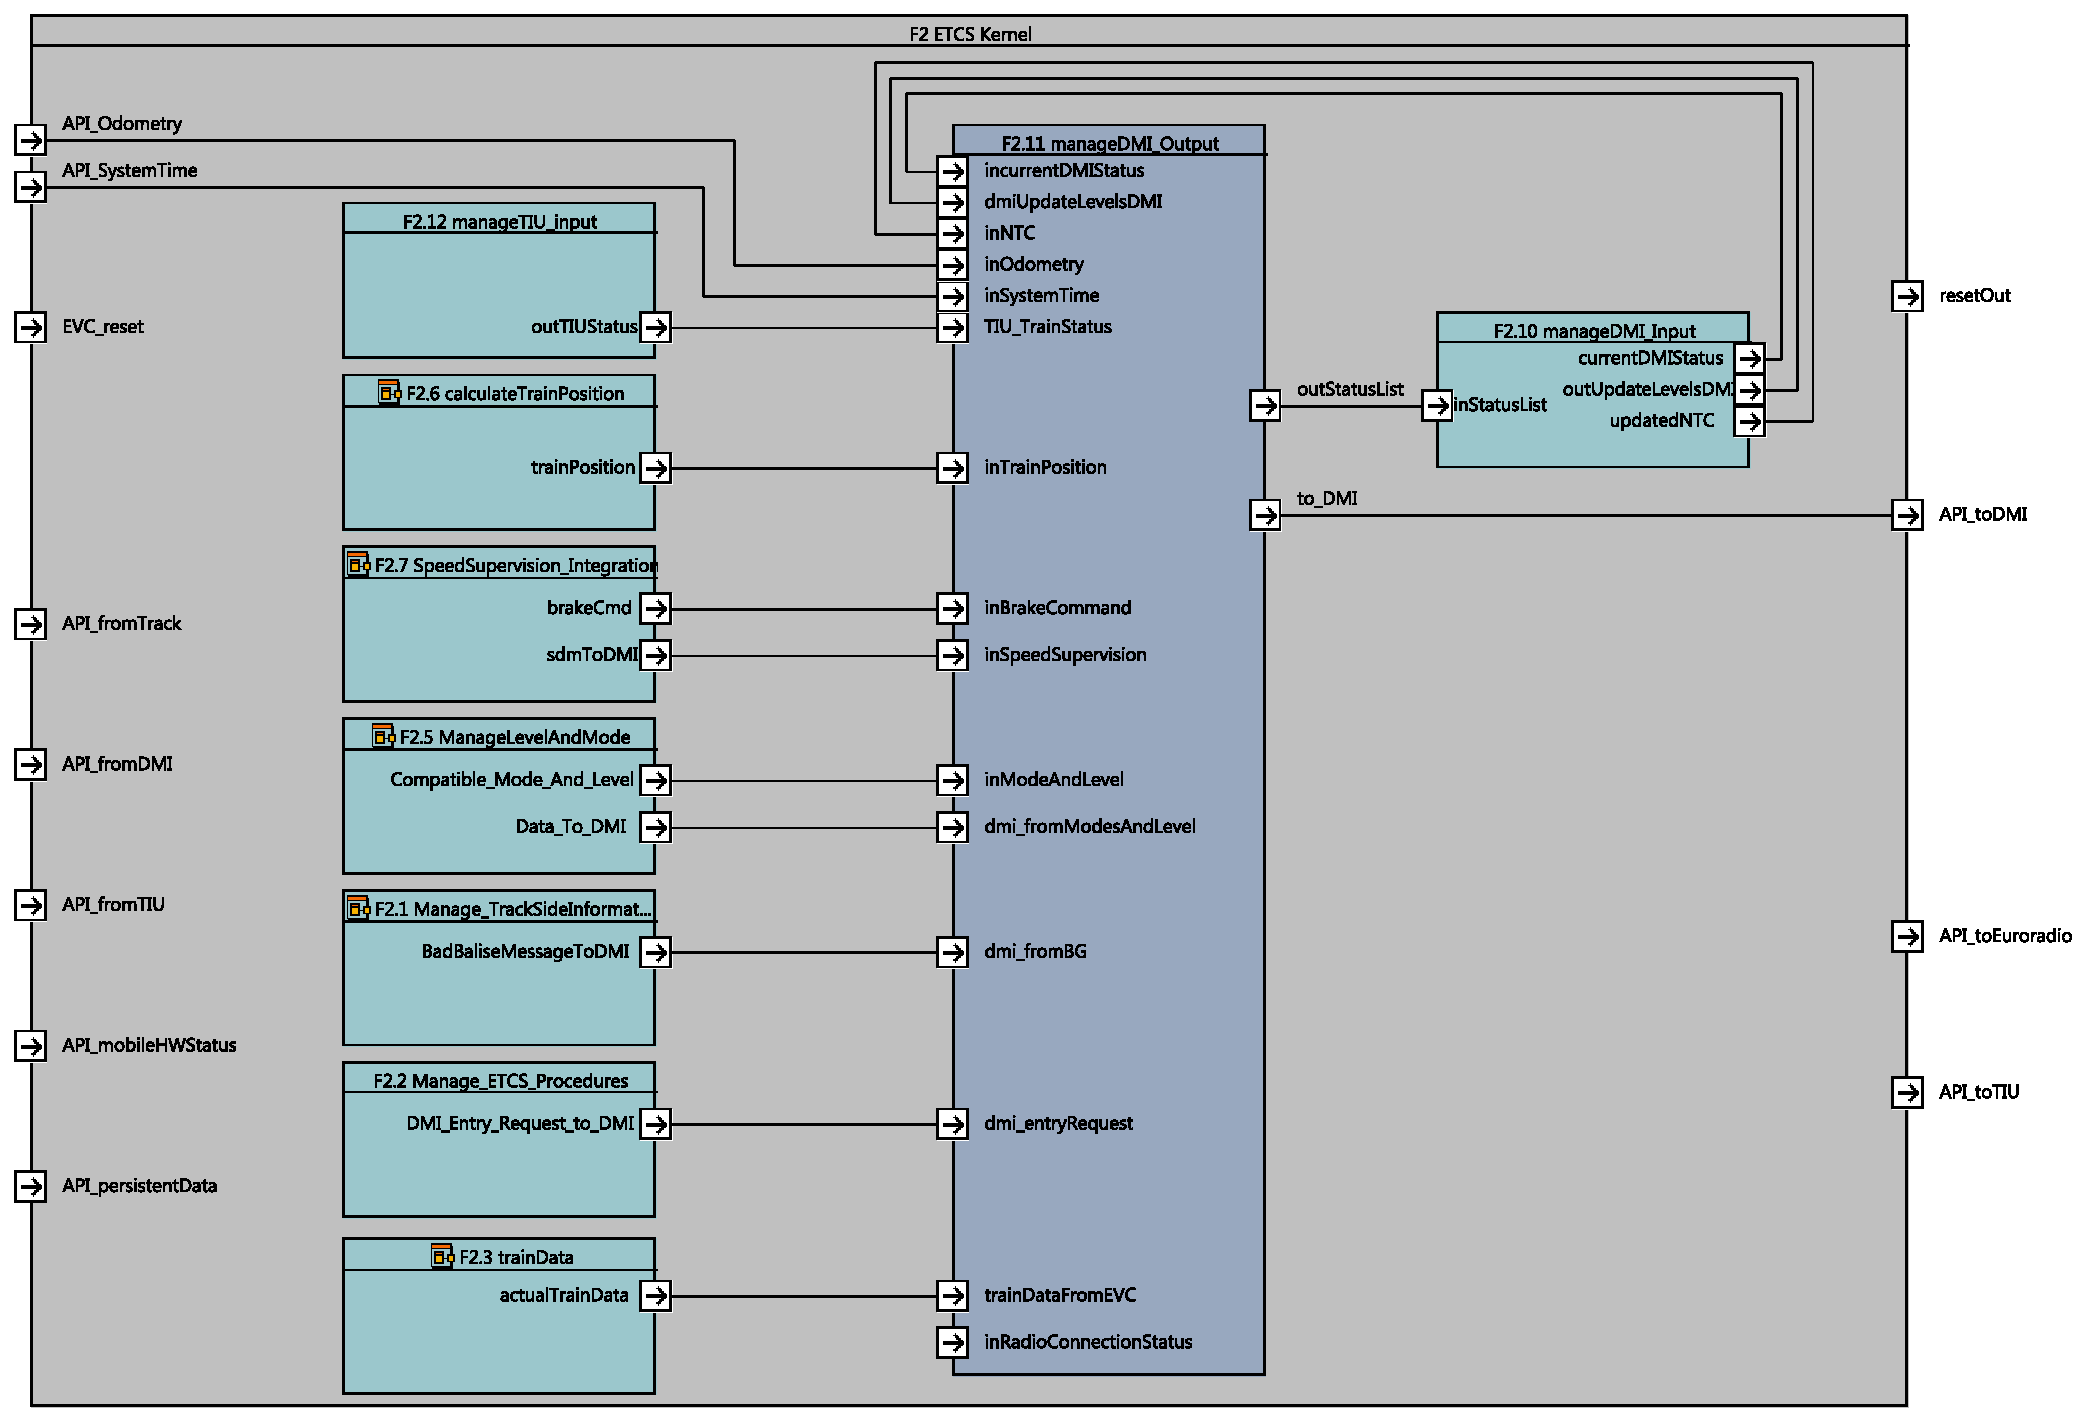
\includegraphics[width=\textwidth]{F2_F2_11.pdf}
\caption{F2: ETCS Kernel SysML diagram with focus on F2.11 ManageDMIOutput component.}\label{f:f2.11_overview}
\end{figure}

\begin{figure}
\center
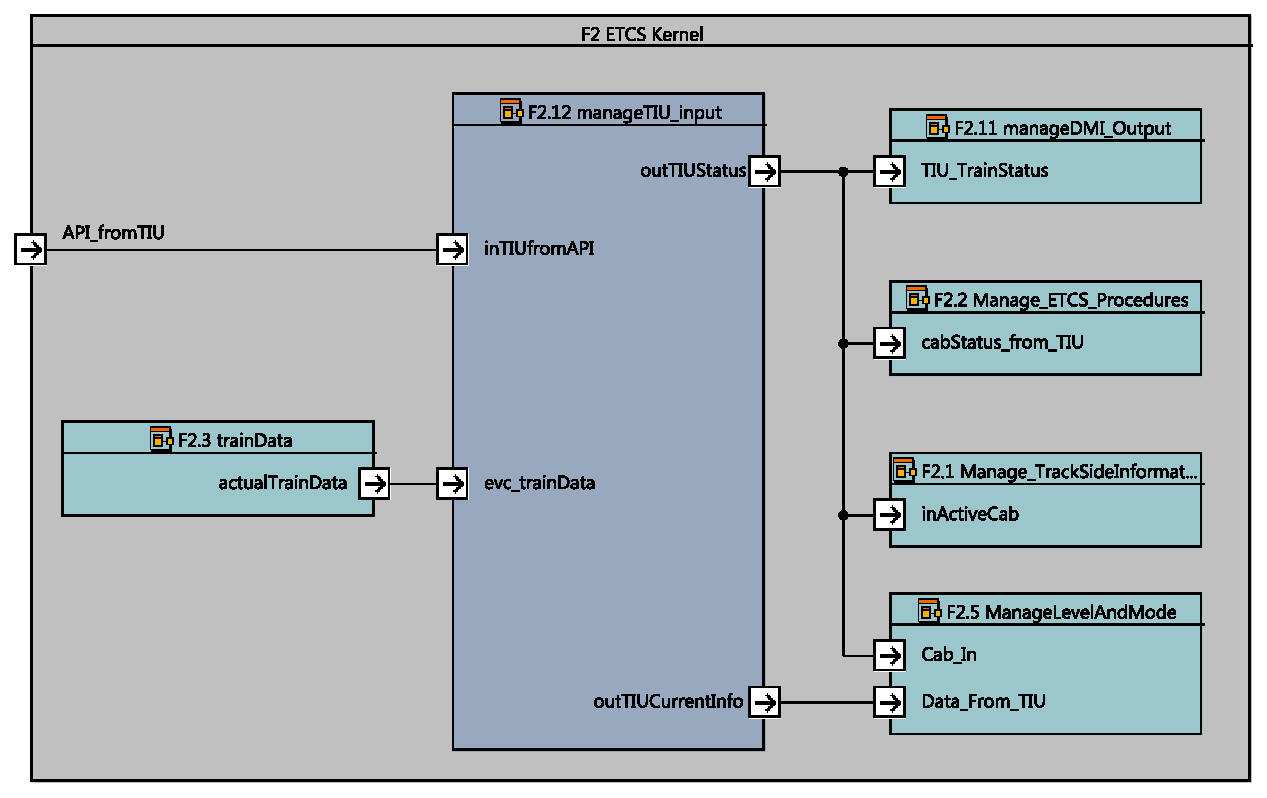
\includegraphics[width=\textwidth]{F2_F2_12.pdf}
\caption{F2: ETCS Kernel SysML diagram with focus on F2.12 ManageTIUInput component.}\label{f:f2.12_overview}
\end{figure}

\begin{figure}
\center
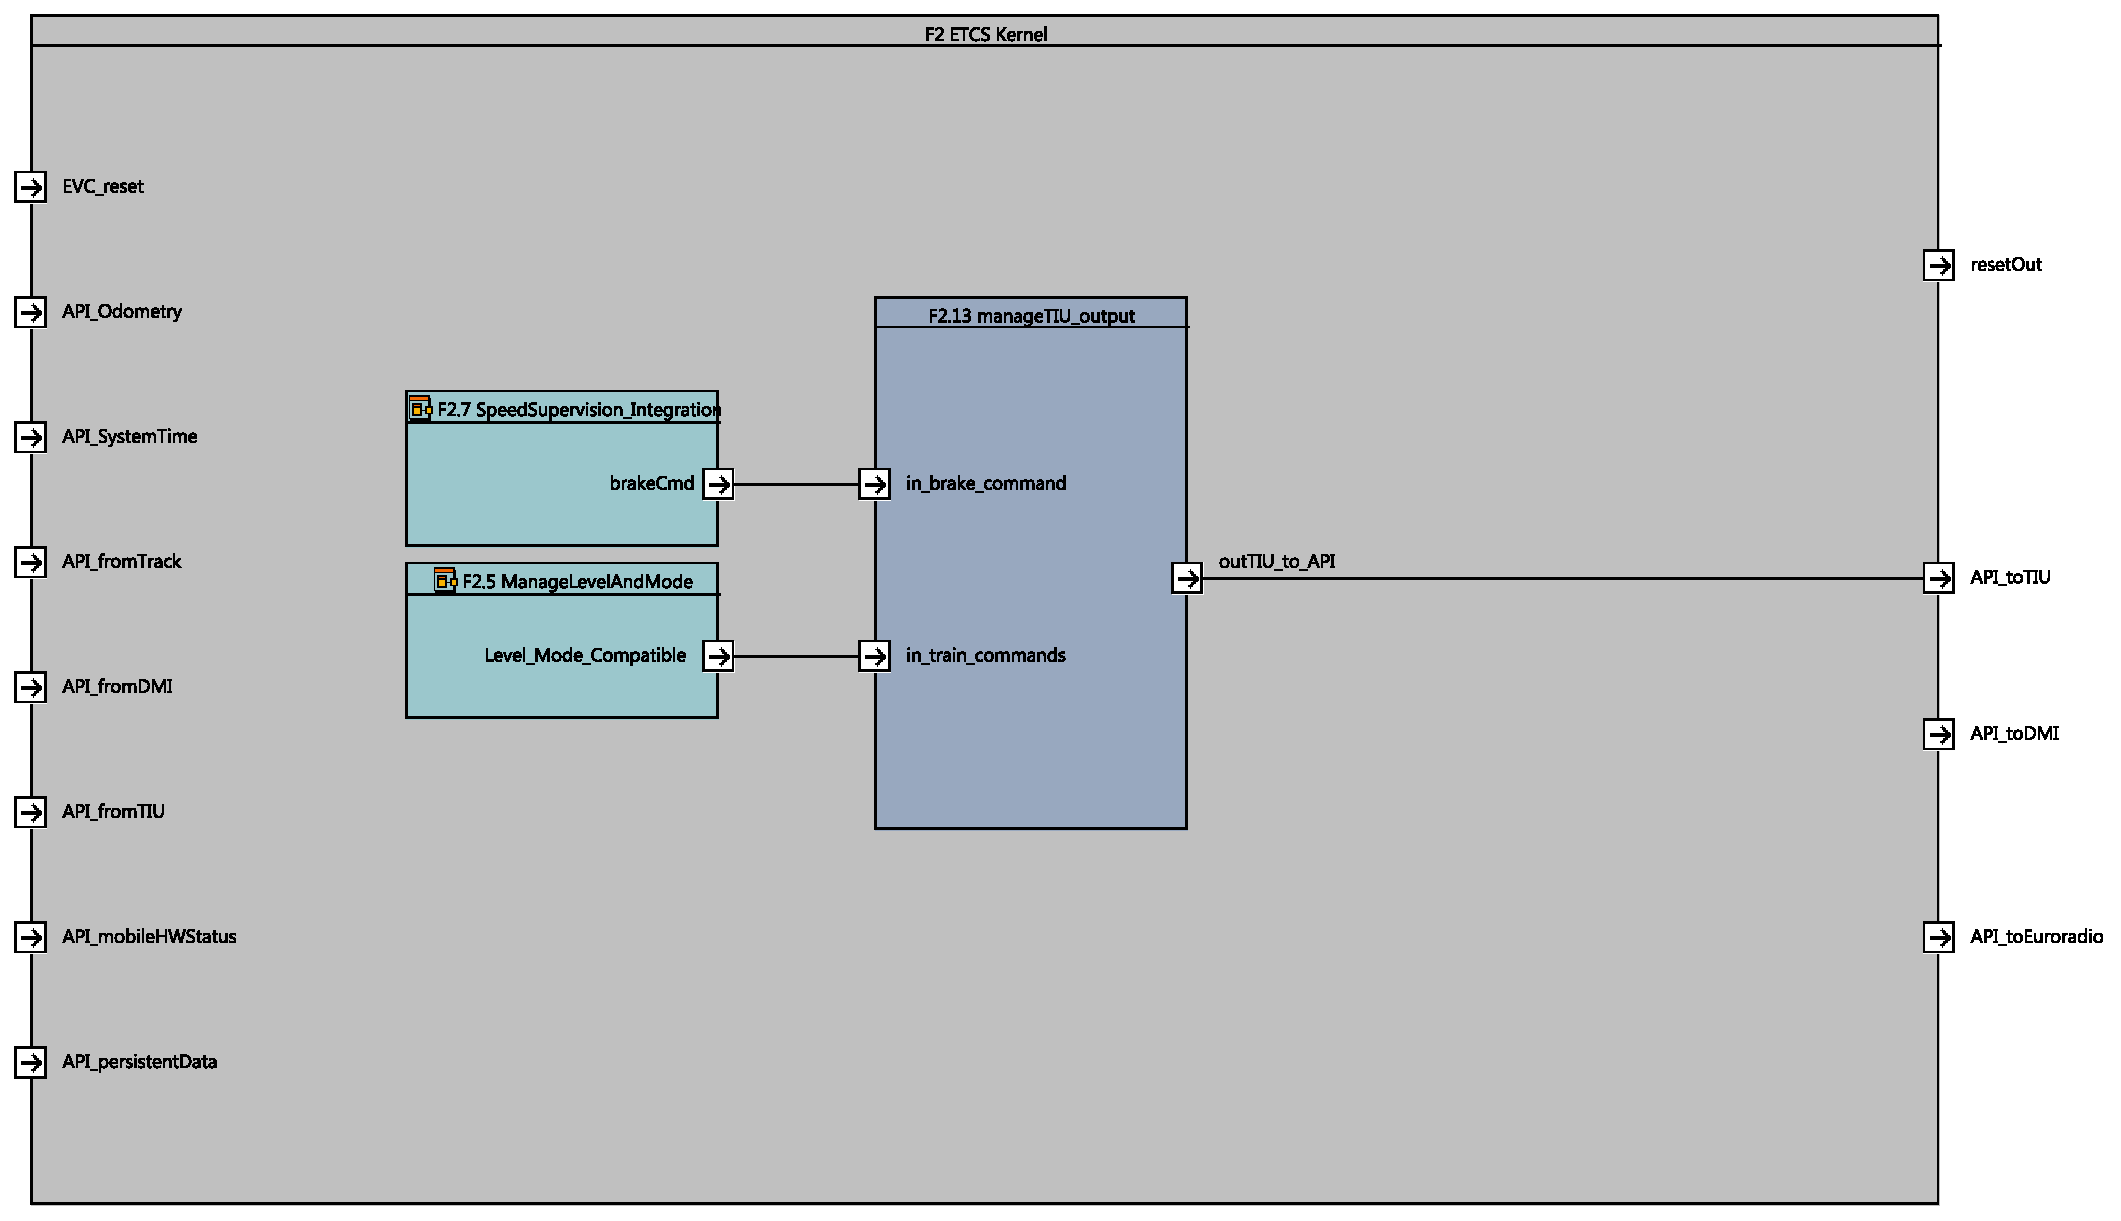
\includegraphics[width=\textwidth]{F2_F2_13.pdf}
\caption{F2: ETCS Kernel SysML diagram with focus on F2.13 ManageTIUOutput component.}\label{f:f2.13_overview}
\end{figure}
















\subsection{External Interfaces}
This section gives a detailed overview of the external inputs and outputs of module F2: ETCS Kernel.

\subsubsection{External Inputs}

\paragraph{EVC\_reset}

\begin{longtable}{p{.25\textwidth}p{.7\textwidth}}
\toprule
Input name				& EVC\_reset \\
\midrule
Description				&  The reset input is used to delete all data stored in the connected components inside F2 (e.g.~collected balise telegrams). If the input is set to true, all data kept in the components is deleted and no input is accepted. The reset option is to be used when the EVC is started or in system error scenarios. \\
\midrule
Source					& System Startup and Recovery\\ 
\midrule
Type					& bool \\
\midrule
Valid range of values	&
\begin{description}
\item [true]: evc needs to be reset. All stored data of subcomponents get reset by there functions. evc needs to restart with a start of mission procedure.
\item [false]: no reset of the unit.
\end{description}
\\
\midrule
Behaviour when value is at boundary	& not applicable \\
\midrule
Behaviour for values out of valid range	& not applicable \\
\midrule
Behaviour when value is erroneous, absent or unwanted (i.e. spurious) &not applicable \\
\bottomrule
\end{longtable}

\paragraph{API\_Odometry}

\begin{longtable}{p{.25\textwidth}p{.7\textwidth}}
\toprule
Input name				& API\_Odometry \\
\midrule
Description				& Odometry data provided by the external odometry module of the train. \\
\midrule
Source					& Odometer Unit\\ 
\midrule
Type					& structure \\
\midrule
Valid range of values	& n.a. \\
\midrule
Behaviour when value is at boundary	& n.a. \\
\midrule
Behaviour for values out of valid range	& n.a. \\
\midrule
Behaviour when value is erroneous, absent or unwanted (i.e. spurious) &n.a. \\
\bottomrule
\end{longtable}

\paragraph{API\_SystemTime}

\begin{longtable}{p{.25\textwidth}p{.7\textwidth}}
\toprule
Input name				& API\_SystemTime \\
\midrule
Description				& System time as defined by the runtime system. \\
\midrule
Source					& evc operating system  \\ 
\midrule
Type					& int \\
\midrule
Valid range of values	& positive range of int\\
\midrule
Behaviour when value is at boundary	& reset of the time. \\
\midrule
Behaviour for values out of valid range	& may result in loss of rbc messages dur to sequencing errors and finally to the loss of an active radio connection. As a result train may go into standstill caused by emergency brake \\
\midrule
Behaviour when value is erroneous, absent or unwanted (i.e. spurious) & see above \\
\bottomrule
\end{longtable}

\paragraph{API\_fromTrack}

\begin{longtable}{p{.25\textwidth}p{.7\textwidth}}
\toprule
Input name				& API\_fromTrack \\
\midrule
Description				& Messages and Telegrams from trackside. \\
\midrule
Source					& BTM resp. RTM\\ 
\midrule
Type					& structure \\
\midrule
Valid range of values	& n.a. \\
\midrule
Behaviour when value is at boundary	& n.a. \\
\midrule
Behaviour for values out of valid range	& n.a. \\
\midrule
Behaviour when value is erroneous, absent or unwanted (i.e. spurious) & n.a. \\
\bottomrule
\end{longtable}

\paragraph{API\_fromDMI}

\begin{longtable}{p{.25\textwidth}p{.7\textwidth}}
\toprule
Input name				& API\_fromDMI \\
\midrule
Description				& Input message from DMI \\
\midrule
Source					& API respectively F6 DMI Controller\\ 
\midrule
Type					& structure \\
\midrule
Valid range of values	& n.a. \\
\midrule
Behaviour when value is at boundary	& n.a. \\
\midrule
Behaviour for values out of valid range	& n.a. \\
\midrule
Behaviour when value is erroneous, absent or unwanted (i.e. spurious) & n.a. \\
\bottomrule
\end{longtable}

\paragraph{API\_fromTIU}

\begin{longtable}{p{.25\textwidth}p{.7\textwidth}}
\toprule
Input name				& API\_fromTIU \\
\midrule
Description				& Input message from the TIU \\
\midrule
Source					& API respectively F7 Manage TIU Interface \\ 
\midrule
Type					& structure \\
\midrule
Valid range of values	& n.a. \\
\midrule
Behaviour when value is at boundary	& n.a. \\
\midrule
Behaviour for values out of valid range	& n.a. \\
\midrule
Behaviour when value is erroneous, absent or unwanted (i.e. spurious) & n.a. \\
\bottomrule
\end{longtable}

\paragraph{API\_mobileHWStatus}

\begin{longtable}{p{.25\textwidth}p{.7\textwidth}}
\toprule
Input name				& API\_mobileHWStatus \\
\midrule
Description				& Actual status of the connected radio module. This implementation is based on a single radio module. The upgrade to a system with 2 mobiles is in preparation.\\
\midrule
Source					& RTM \\ 
\midrule
Type					& structure \\
\midrule
Valid range of values	& n.a. \\
\midrule
Behaviour when value is at boundary	& n.a. \\
\midrule
Behaviour for values out of valid range	& n.a. \\
\midrule
Behaviour when value is erroneous, absent or unwanted (i.e. spurious) & n.a. \\
\bottomrule
\end{longtable}

\paragraph{API\_persistentData}

\begin{longtable}{p{.25\textwidth}p{.7\textwidth}}
\toprule
Input name				& API\_persistentData \\
\midrule
Description				& Storage of data which need to be loaded in order to be able to start the start of mission procedure. The data has to be saved as a part of the end of mission procedure. \\
\midrule
Source					& evc-Storage \\ 
\midrule
Type					& structure \\
\midrule
Valid range of values	& n.a. \\
\midrule
Behaviour when value is at boundary	& n.a. \\
\midrule
Behaviour for values out of valid range	& n.a. \\
\midrule
Behaviour when value is erroneous, absent or unwanted (i.e. spurious) &n.a. \\
\bottomrule
\end{longtable}



\subsubsection{External Outputs}

\paragraph{resetOut}

\begin{longtable}{p{.25\textwidth}p{.7\textwidth}}
\toprule
Output name				& resetOut \\
\midrule
Description				& Indicator for the succesful execution of the reset function for the evc. \\
\midrule
Destination				& System Startup and Recovery \\ 
\midrule
Type					& bool \\
\midrule
Valid range of values	& true: ok, false: not ok \\
\midrule
Behaviour when value is at boundary	& n.a. \\
\midrule
Behaviour for values out of valid range	& n.a. \\
\midrule
Behaviour when value is erroneous, absent or unwanted (i.e. spurious) & n.a. \\
\bottomrule
\end{longtable}


\paragraph{API\_toEuroradio}

\begin{longtable}{p{.25\textwidth}p{.7\textwidth}}
\toprule
Output name				& API\_toEuroradio \\
\midrule
Description				& Radio Messages to be sent to the RBC. The output is dedicated to a sending RTM module. In addition to the messages, commands for controlling the Radio module are implemented in this interface  \\
\midrule
Destination				& Radio Module (RTM) \\ 
\midrule
Type					& structure \\
\midrule
Valid range of values	& n.a. \\
\midrule
Behaviour when value is at boundary	& n.a. \\
\midrule
Behaviour for values out of valid range	& n.a. \\
\midrule
Behaviour when value is erroneous, absent or unwanted (i.e. spurious) &n.a. \\
\bottomrule
\end{longtable}


\paragraph{API\_toDMI}

\begin{longtable}{p{.25\textwidth}p{.7\textwidth}}
\toprule
Output name				& API\_toDMI \\
\midrule
Description				& Messages to be sent to the DMI \\
\midrule
Destination				& API respectively F6DMI Controller \\ 
\midrule
Type					& structure\\
\midrule
Valid range of values	& n.a. \\
\midrule
Behaviour when value is at boundary	& n.a. \\
\midrule
Behaviour for values out of valid range	& n.a.\\
\midrule
Behaviour when value is erroneous, absent or unwanted (i.e. spurious) & n.a.\\
\bottomrule
\end{longtable}

\paragraph{API\_toTIU}

\begin{longtable}{p{.25\textwidth}p{.7\textwidth}}
\toprule
Output name				& API\_toTIU \\
\midrule
Description				& Interface to the train Interface Unit (TIU) including Brake Interface Unit (BIU) \\
\midrule
Destination				& API respectively F7 Manage TIU Interface \\ 
\midrule
Type					& structure \\
\midrule
Valid range of values	& n.a. \\
\midrule
Behaviour when value is at boundary	& n.a. \\
\midrule
Behaviour for values out of valid range	& n.a.\\
\midrule
Behaviour when value is erroneous, absent or unwanted (i.e. spurious) & n.a. \\
\bottomrule
\end{longtable}